% =================================================================================================
% set document class
% =================================================================================================
\documentclass[mathserif,dvipsnames,table,xcdraw]{beamer}

% =================================================================================================
% packages
% =================================================================================================
\usepackage{animate}
\usepackage{multicol}
\usepackage{algorithm}
\usepackage{algpseudocode}
\usepackage{amsmath}
\usepackage{amssymb}
\usepackage{amsthm}
\usepackage{mathtools}
\usepackage{bm}
\usepackage[utf8]{inputenc}
\usepackage[english]{babel}
\usepackage[T1]{fontenc}
\usepackage{tcolorbox}
\RequirePackage{fix-cm}


% =================================================================================================
% set mode and theme
% =================================================================================================
\mode<presentation>{\usetheme{Antibes}}

% =================================================================================================
% input definitions 
% =================================================================================================
%% math defs.tex
\newcommand{\ones}{\mathbf 1}
\newcommand{\reals}{{\mbox{\bf R}}}
\newcommand{\integers}{{\mbox{\bf Z}}}
\newcommand{\symm}{{\mbox{\bf S}}}  % symmetric matrices

\newcommand{\nullspace}{{\mathcal N}}
\newcommand{\range}{{\mathcal R}}
\newcommand{\Rank}{\mathop{\bf Rank}}
\newcommand{\Tr}{\mathop{\bf Tr}}
\newcommand{\diag}{\mathop{\bf diag}}
\newcommand{\card}{\mathop{\bf card}}
\newcommand{\rank}{\mathop{\bf rank}}
\newcommand{\conv}{\mathop{\bf conv}}
\newcommand{\prox}{\mathbf{prox}}

\newcommand{\Expect}{\mathop{\bf E{}}}
\newcommand{\Prob}{\mathop{\bf Prob}}
\newcommand{\Co}{{\mathop {\bf Co}}} % convex hull
\newcommand{\dist}{\mathop{\bf dist{}}}
\newcommand{\argmin}{\mathop{\rm argmin}}
\newcommand{\argmax}{\mathop{\rm argmax}}
\newcommand{\epi}{\mathop{\bf epi}} % epigraph
\newcommand{\Vol}{\mathop{\bf vol}}
\newcommand{\dom}{\mathop{\bf dom}} % domain
\newcommand{\intr}{\mathop{\bf int}}
\newcommand{\sign}{\mathop{\bf sign}}

\newcommand{\cf}{{\it cf.}}
\newcommand{\eg}{{\it e.g.}}
\newcommand{\ie}{{\it i.e.}}
\newcommand{\etc}{{\it etc.}}
%% define some colors (generated for Antibes)
\definecolor{PERSIAN_BLUE}{RGB}{51,51,178}
\definecolor{RAISIN_BLACK}{RGB}{42,45,52}
\definecolor{RUSSIAN_GREEN}{RGB}{92,148,110}
\definecolor{GREEN_SHEEN}{RGB}{128,194,175}
\definecolor{BLIZZARD_BLUE}{RGB}{160,221,230}
\definecolor{DARK_ORANGE}{RGB}{255,143,41}
\definecolor{PICOTEE_BLUE}{RGB}{38,38,134}
\definecolor{BISTRE}{RGB}{55,44,37}
\definecolor{GRAY_WEB}{RGB}{131,131,131}
\definecolor{DARK_SKY_BLUE}{RGB}{147,183,190}
\definecolor{MINT_CREAM_1}{RGB}{241,255,250}
\definecolor{MINT_CREAM_2}{RGB}{247,255,247}
\definecolor{PALE_SILVER}{RGB}{213,199,188}
\definecolor{OPAL}{RGB}{148,191,190}
\definecolor{CELADON}{RGB}{172,247,193}
\definecolor{LASER_LEMON}{RGB}{252,252,98}
\definecolor{MINDARO}{RGB}{218,255,125}
\definecolor{GRANNY_SMITH_APPLE}{RGB}{178,239,155}
\definecolor{RHYTHM}{RGB}{140,134,170}
\definecolor{SILVER}{RGB}{197,197,197}
\definecolor{SPANISH_GRAY_1}{RGB}{130,145,145}
\definecolor{SPANISH_GRAY_2}{RGB}{148,155,150}
\definecolor{BRICK_RED}{RGB}{195,60,84}
\definecolor{SKY_BLUE_CRAYOLA}{RGB}{142,227,239}
\definecolor{CELESTE}{RGB}{174,243,231}
\definecolor{HOOKERS_GREEN}{RGB}{88,125,113}
\definecolor{GREEN_PANTONE}{RGB}{77,170,87}
\definecolor{NAPLES_YELLOW}{RGB}{255,130,109}
\definecolor{AIR_SUPERIORITY_BLUE}{RGB}{108,166,193}
\definecolor{FIRE_BRICK}{RGB}{179,0,27}
\definecolor{ICE_BERG}{RGB}{126,163,204}
\definecolor{TAN}{RGB}{204,173,143}
\definecolor{MIDDLE_BLUE}{RGB}{247,255,247}
\definecolor{LAVENDER_BLUSH}{RGB}{238,229,233}
\definecolor{CINNABAR}{RGB}{214,73,51}
\definecolor{BABY_POWDER}{RGB}{247,247,242}
\definecolor{AQUA_MARINE}{RGB}{133,255,199}
\definecolor{CORAL}{RGB}{255,133,82}
\definecolor{PLATINUM}{RGB}{230,230,230}
\definecolor{BROWN}{RGB}{126,89,32}
\definecolor{FULVOUS}{RGB}{220,133,31}
\definecolor{YELLOW_ORANGE}{RGB}{255,167,55}
\definecolor{GLOSSY_GRAPE}{RGB}{171,146,191}
\definecolor{BITTER_SWEET}{RGB}{255,111,89}
\definecolor{ZOMP}{RGB}{67,170,139}
\definecolor{AMARANTH_RED}{RGB}{215,29,45}
\definecolor{SPACE_CADET}{RGB}{49,61,90}
\definecolor{CELADON_BLUE}{RGB}{66,129,164}
\definecolor{ELECTRIC_BLUE}{RGB}{142, 237, 247}
\definecolor{BABY_BLUE_EYES}{RGB}{161, 205, 241}
\definecolor{STAR_COMMAND}{RGB}{34, 116, 165}
\definecolor{DENIM_BLUE}{RGB}{57, 67, 183}
\definecolor{BLUE_JEANS}{RGB}{72, 172, 240}
\definecolor{UPSDELL_RED}{RGB}{180, 24, 37}
\definecolor{RED_MUNSELL}{RGB}{228, 58, 72}
\definecolor{BLUE_MUNSELL}{RGB}{27, 154, 170}
\definecolor{LIBERTY}{RGB}{76, 76, 157}
\definecolor{BABY_BLUE}{RGB}{108, 207, 246}
\definecolor{CAROLINA_BLUE}{RGB}{27, 152, 224}
\definecolor{PORTLAND_ORANGE}{RGB}{244, 96, 54}
\definecolor{MINION_YELLOW}{RGB}{242, 220, 93}
\definecolor{SANDY_BROWN}{RGB}{242, 163, 89}
\definecolor{FLAME}{RGB}{215, 78, 9}
\definecolor{BLOOD_RED}{RGB}{110, 14, 10}
\definecolor{CLARET}{RGB}{137, 4, 61}
\definecolor{EMERALD}{RGB}{68, 207, 108}
\definecolor{ILLUMINATING_EMERALD}{RGB}{50, 147, 111}
\definecolor{MAROON_X_11}{RGB}{184, 19, 101}
\definecolor{CARRIBEAN_GREEN}{RGB}{29, 211, 176}
\definecolor{RED_CRAYOLA}{RGB}{239, 45, 86}
\definecolor{MIKADO_YELLOW}{RGB}{255, 193, 0}
\definecolor{SELECTIVE_YELLOW}{RGB}{255, 186, 8}
\definecolor{MISTY_ROSE}{RGB}{255, 227, 220}
\definecolor{HONEY_YELLOW}{RGB}{247, 179, 43}




% =================================================================================================
% new command definitions 
% =================================================================================================
\newcommand{\fnt}[1]{\fontsize{#1}{0}\selectfont}

% =================================================================================================
% title
% =================================================================================================
\title[\textbf{How good is the Bayes Posterior in Deep neural Networks really?}]{
	\textbf{How good is the Bayes Posterior in Deep Neural Networks really?}
}
\subtitle{Wenzel, Florian and Roth, Kevin and Veeling, Bastiaan S and {\'S}wi{\k{a}}tkowski, Jakub and Tran, Linh and Mandt, Stephan and Snoek, Jasper and Salimans, Tim and Jenatton, Rodolphe and Nowozin, Sebastian}
\author{\textcolor{RAISIN_BLACK}{Presented by: Pritam Karmokar}}
\institute{
	\textcolor{RUSSIAN_GREEN}{\textbf{Bayesian Learning Series (\#11)}} \newline \newline
	\textcolor{DARK_ORANGE}{Robotic Vision Lab (RVL)}\newline 
	\textcolor{BLIZZARD_BLUE}{[Weekly Seminars 03/03/2021]}
}
\date{}


% =================================================================================================
% document
% =================================================================================================
\begin{document}

% -------------------------------------------------------------------------------------------------
% title 
% -------------------------------------------------------------------------------------------------
%% title frame
\begin{frame}
	\titlepage
\end{frame}

% -------------------------------------------------------------------------------------------------
% table of contents 
% -------------------------------------------------------------------------------------------------
%% ToC
\begin{frame}{Outline}
	\tableofcontents
\end{frame}

%% ToC at beginning of sections
\AtBeginSection[]
{
\begin{frame}{Outline}
	\tableofcontents[currentsection]
\end{frame}
}

%% ToC at beginning of subsections
\AtBeginSubsection[]
{
\begin{frame}{Outline}
	\tableofcontents[currentsubsection]
\end{frame}
}


% -------------------------------------------------------------------------------------------------
% introduction 
% -------------------------------------------------------------------------------------------------

\section[Introduction]{Introduction}
\label{sec:introduction}

	\begin{frame}{Introduction}
		{(in the past five years)}
		\textbf{Inference procedures} have been developed that allow for \textbf{Bayesian inference in Deep Neural Networks}
		\begin{itemize}
			\item<2-> Increasingly accurate 
			\item<3-> Efficiently approximate
			\only<4->{\\
			\vspace{1ex} \hspace{5ex} \fnt{20}{+} 
			}
			\item<4-> Algorithmic progress
			\item<5-> Improved uncertainty quantification \only<6->{and sample efficiency}
		\end{itemize}		
	\end{frame}

	\begin{frame}{Introduction}
		{(as of early 2020)}
		Despite all that, ..
		\begin{itemize}
			\item<2-> \textbf{No publicized deployments} of Bayesian neural networks \textbf{in industrial practice}
			\only<3->{\\
			\vspace{5ex} \hspace{25ex} \textcolor{DARK_ORANGE}{\textbf{\fnt{20}{?}}}
			}
		\end{itemize}
	\end{frame}

	\begin{frame}{Introduction}
		{\ ?..}
		Cast doubts on,
		\begin{itemize}
			\item<2-> \textbf{current understanding} of Bayes posteriors in popular deep neural networks
		\end{itemize}
	\end{frame}

	\begin{frame}{Introduction}
		\textbf{Demonstrate} through careful MCMC sampling
		\begin{itemize}
			\item<2-> Bayesian posterior predictives yield \textbf{systematically worse predictions} compared to simpler methods (\textit{e.g., point estimates obtained from SGD})
			\item<3-> predictive performance \textbf{improved through use of a cold posterior} that \textcolor{MAROON_X_11}{overcounts evidence}.
		\end{itemize}
	\end{frame}

	\begin{frame}{Introduction}
		\begin{itemize}
			\item \textbf{Demonstrate} through careful MCMC sampling
			\item<2-> \textbf{Put forward} several hypotheses that could explain cold posteriors
			\item<3-> \textbf{Evaluate} hypotheses through experiments
			\item <4-> \textbf{Question} the goal of accurate posterior approximations in Bayesian Deep Learning
		\end{itemize}
	\end{frame}

	\begin{frame}{Introduction}
		{Question the goal of accurate posterior approximations}
		\begin{itemize}
			\item If the true Bayes posterior is poor, \only<1>{..}\only<2->{\textbf{what is the use of more accurate approximations?}}
			\item<3-> \textbf{Time to focus} on understanding of \textbf{origin of improved performance of cold posteriors}
		\end{itemize}
	\end{frame}

	\begin{frame}{Introduction}
		In supervised learning, we use
		\begin{itemize}
			\item<2-> training dataset $\mathcal{D} = \left\{x_i, y_i\right\}_{i=1,\ldots,n}$
			\item<3-> probabilistic model $p(y\vert x, \bm{\theta})$
			\item <4-> to minimize regularized cross-entropy objective
			\begin{equation}
				\label{eqn:cross_ent_obj}
				L(\bm{\theta}) \coloneqq  - \frac{1}{n}\sum\limits_{i=1}^{n} \log p\left(y_i \vert x_i, \bm{\theta}\right) + \Omega(\bm{\theta})
			\end{equation}
		\end{itemize}
	\end{frame}
\subsection[Bayesian Deep Learning]{Bayesian Deep Learning}
\label{subsec:bayesian_deep_learning}
	\begin{frame}{Bayesian Deep Learning}
		{}
		\begin{itemize}
			\item do \textbf{not} optimize for a \textbf{\textit{single}} likely model
			\item <3->instead want to discover \textbf{\textit{all}} likely models
			\item <4-> \textbf{approximate} the \textbf{\textit{posterior distribution}} over model parameters, $p(\bm{\theta}\vert \mathcal{D}) \propto exp(-$\only<5->{\textcolor{CINNABAR}}{$U(\bm{\theta})$}$/T)$\only<5->{, where \only<5->{\textcolor{CINNABAR}}{$U(\bm{\theta})$} is the \textbf{\textit{posterior energy function}},
			\begin{equation}
				\label{eqn:posterior_energy_function}
				U(\bm{\theta}) \coloneqq -\sum\limits_{i=1}^{n} \log p\left(y_i \vert x_i, \bm{\theta}\right) - \log p(\bm{\theta})
			\end{equation}
			}
		\end{itemize}
	\end{frame}

	\begin{frame}{Bayesian Deep Learning}
		\begin{itemize}
			\only<-2>{
				\item Given $p(\bm{\theta}\vert \mathcal{D})$, we \textit{predict} on a new instance $x$, by averaging over all likely models,
				\begin{equation}
					\label{eqn:bayes_ensemble}
					p(y\vert x,\mathcal{D}) = \int p(y\vert x,\bm{\theta}) p(\bm{\theta}\vert \mathcal{D}) d\bm{\theta},
				\end{equation}
			}
			\only<2>{where (\ref{eqn:bayes_ensemble}) is also known as \textbf{\textit{posterior predictive}} or \textbf{\textit{Bayes ensemble}}.}
			\item<3-> solving (\ref{eqn:bayes_ensemble}) exactly is not possible
			\item <4-> instead approximate it using sample approximation $p(y\vert x,\mathcal{D}) \approx \frac{1}{S}\sum\nolimits_{s=1}^{S} p(y \vert x, $ \only<5->{\textcolor{CINNABAR}}{${\bm{\theta}}^{(s)}$}$)$\only<5->{, where \only<5->{\textcolor{CINNABAR}}{${\bm{\theta}}^{(s)}$} is approximately sampled from $p(\bm{\theta}\vert \mathcal{D})$}
		\end{itemize}
	\end{frame}

	\begin{frame}{Bayesian Deep Learning}
		{\textit{the suprising effect called the "Cold Posterior" effect}}
		\begin{tcolorbox}
			\textbf{Cold Posteriors:} among all temperized posteriors the best posterior predictive performance on holdout data is achieved at temperature T < 1. 
		\end{tcolorbox}
		\only<2->{
			\centering
			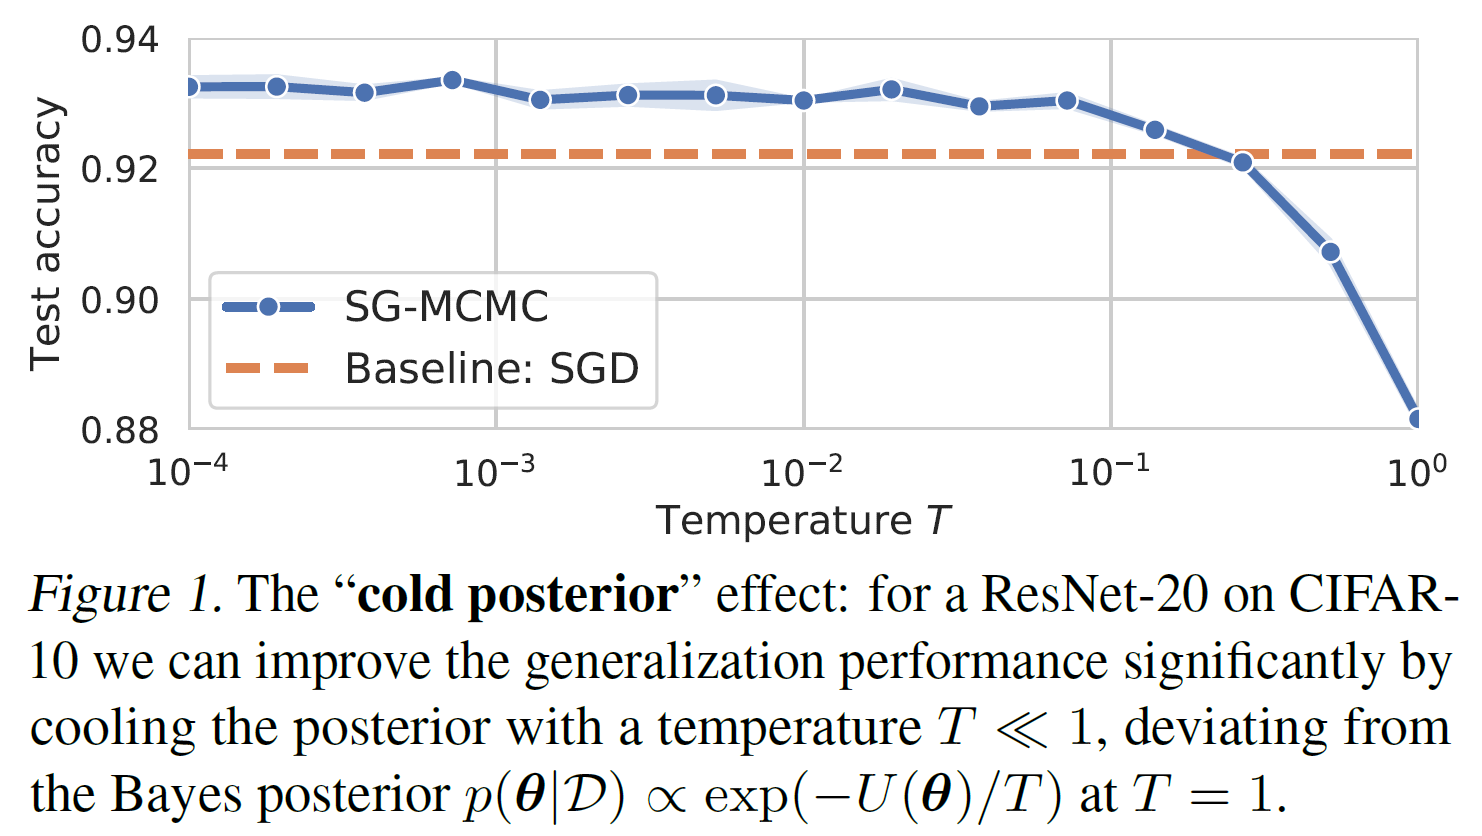
\includegraphics[width=0.6\textwidth]{../figures/cold_post_1.png}
		}
	\end{frame}

\subsection[Why should Bayes ($T=1$) be better?]{Why should Bayes ($T=1$) be better?}
\label{subsec:why_bayes_better}

	\begin{frame}{Why should Bayes ($T=1$) be better?}
		\only<1>{Why expect that predictions made by the \textit{ensemble model} (\ref{eqn:bayes_ensemble}) could improve over predictions made at a single well-chosen parameter?}
		\only<2->{
			Three reasons:
			\begin{itemize}
				\item<2->\textbf{\textit{Theory}}: known that (\ref{eqn:bayes_ensemble}) can dominate common point-wise estimators based on likelihood, even in case of misspecification
				\item <3->\textbf{\textit{Classical empirical evidence}}: for classical statistical models, averaged predictions (\ref{eqn:bayes_ensemble}) have been observed to be more robust in practice
				\item <4-> \textbf{\textit{Model averaging}}:recent deep learning models based on deterministic model averages have shown good predictive performance
			\end{itemize}
		}
	\end{frame}

	\begin{frame}{Why should Bayes ($T=1$) be better?}
		\begin{itemize}
			\item <1->Note that a large body of work in Bayesian Deep Learning is \textbf{motivated by the assertion} that predicting \textbf{using (\ref{eqn:bayes_ensemble}) is desirable}
			\item<2-> Authors \textbf{confront the assertion} through \textbf{simple experiments}
			\item<3-> Show that \textbf{our understanding} of the Bayes posterior in deep models \textbf{is limited}
		\end{itemize}
	\end{frame}

	\begin{frame}{Contributions}
		\begin{itemize}
			\item<1-> \textbf{Demonstrate} two models and tasks (ResNet-20 on CIFAR-10 and CNN-LSTM on IMDB) that the Bayes posterior predictive has \textbf{poor performance} compared to SGD-trained models
			\item<2-> \textbf{Put forth and systematically examine hypotheses} that could \textbf{explain the observed behaviour}
			\item<3-> \textbf{Introduce two new diagnostic tools} for assessing the approximation quality of stochastic gradient	Markov chain Monte Carlo methods (SG-MCMC) and \textbf{demonstrate} that the posterior is accurately simulated by existing SG-MCMC methods 
		\end{itemize}
	\end{frame}

\section[Cold Posteriors Perform Better]{Cold Posteriors Perform Better}
\label{sec:cold_posteriors_better}

	\begin{frame}{Deep Learning Models: ResNet-20 and LSTM}
		{ResNet-20 on CIFAR-10}
		\centering
		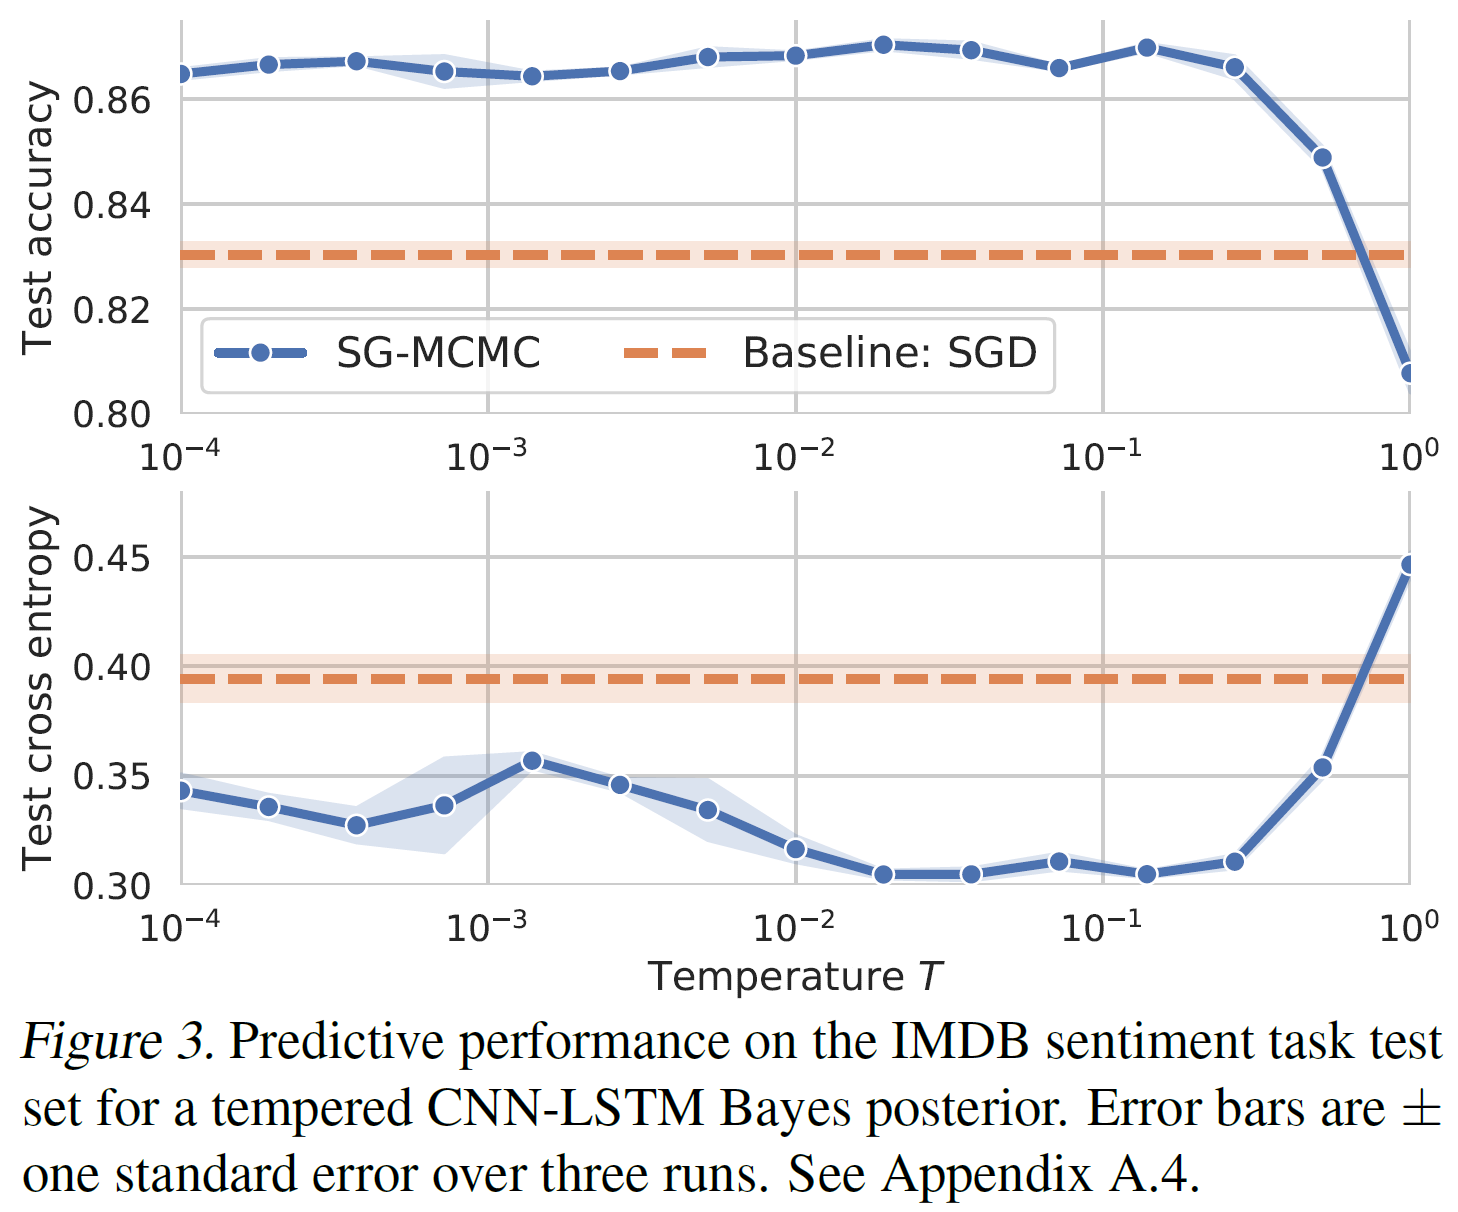
\includegraphics[width=0.6\textwidth]{../figures/imdb_12.png}
	\end{frame}

	\begin{frame}{Deep Learning Models}
		{CNN-LSTM on IMDB text classification}
		\centering
		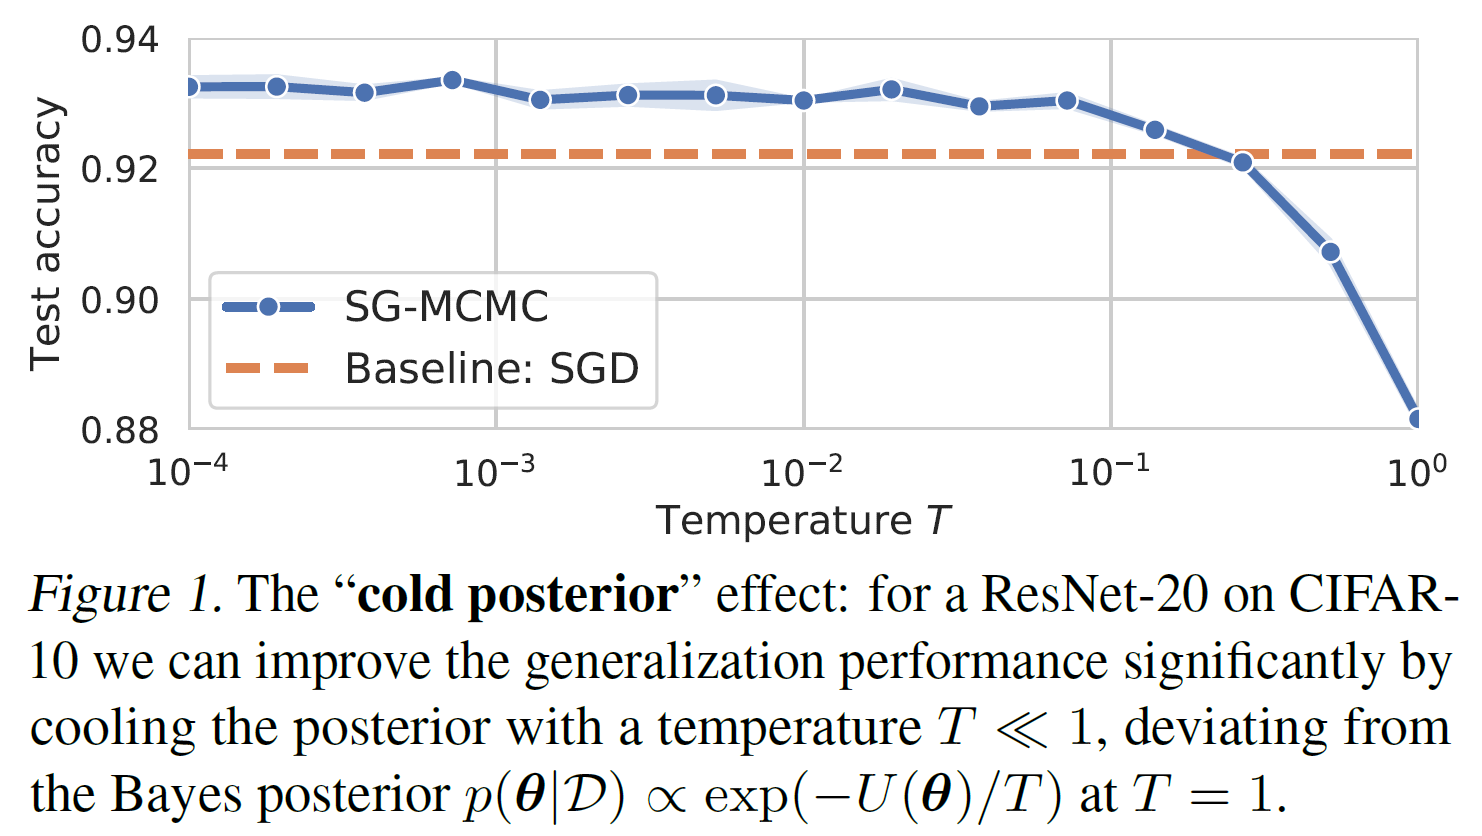
\includegraphics[width=0.4\textwidth]{../figures/cold_post_1.png}
		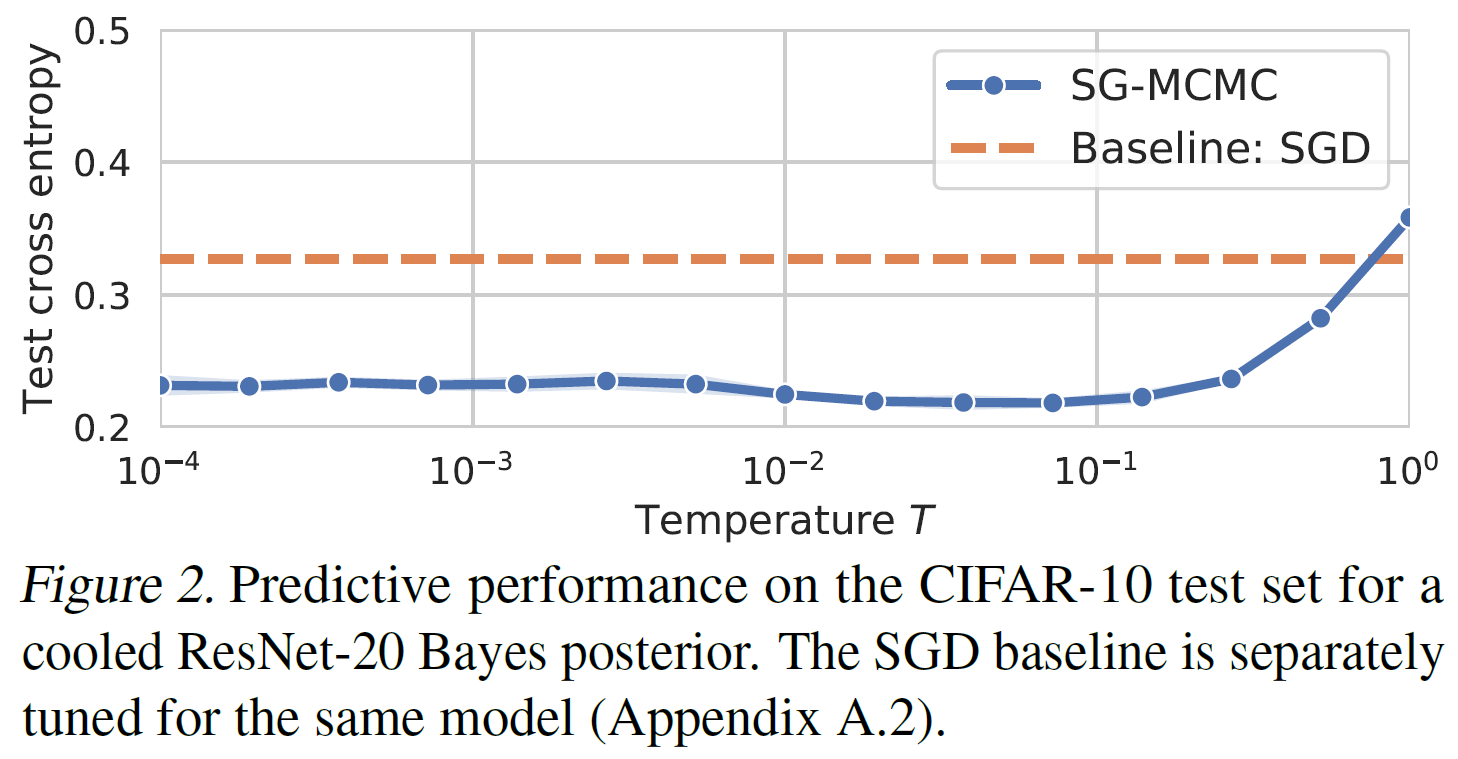
\includegraphics[width=0.4\textwidth]{../figures/cold_post_2.png}
	\end{frame}
	% \begin{frame}{Introduction and Philosophy}
	% 	\begin{itemize}
	% 		\only<1-3>{
	% 		\item Quadrotors inherently \textcolor{GREEN_PANTONE}{active} agents 
	% 		\item Perceptual capabilities in literature mostly \textcolor{DARK_ORANGE}{passive}
	% 		}
	% 		\only<2-3>{
	% 		\item Researchers and practitioners use computer vision algorithms
	% 		\begin{itemize}
	% 			\item To build representations with general capabilities
	% 		\end{itemize}
	% 		}
	% 		\item<3-6> 3D reconstruction of scene + planning
	% 		\item<4-6> Myriad of onboard sensors for 3D modeling environment
	% 		\item<4-6> Gained momentum in recent past 
	% 		\item<5-6> LIDAR, RGB-D and stereo camera 
	% 		\begin{itemize}
	% 			\item<5-6> size, weight, power limitations
	% 		\end{itemize}
	% 		\item<6> Monocular camera with already present IMU
	% 		\item<7-> Full 3D model reconstruction necessary \only<8>{\textcolor{FIRE_BRICK}{..?}} 
	% 	\end{itemize}
	% \end{frame}

	% \begin{frame}{Bio-inspirations for robot design}
	% 	\begin{columns}[totalwidth=0.8\textwidth]
	% 		\begin{column}{0.5\textwidth}
	% 			\centering
	% 			\animategraphics[autoplay,loop,width=0.7\textwidth]{16.66}{../figures/gifs/wildcat/wildcat-}{0}{21}\\
	% 			\animategraphics[autoplay,loop,width=0.7\textwidth]{10}{../figures/gifs/cheetah/cheetah-}{0}{40}\\
	% 			\animategraphics[autoplay,loop,width=0.7\textwidth]{6.66}{../figures/gifs/spider/spider-}{0}{49}
	% 		\end{column}
	% 		\begin{column}{0.5\textwidth}
	% 			\centering
	% 			\animategraphics[autoplay,loop,width=0.7\textwidth]{10}{../figures/gifs/bee/bee-}{0}{19}\\
	% 			\animategraphics[autoplay,loop,width=0.7\textwidth]{6.66}{../figures/gifs/bird/bird-}{0}{33}\\
	% 			\animategraphics[autoplay,loop,width=0.7\textwidth]{15.5}{../figures/gifs/fish/fish-}{0}{33}
	% 		\end{column}
	% 	\end{columns}
	% \end{frame}


	% \begin{frame}{Bio-inspirations for perceptual design - Birds and Insects}
	% 	\begin{itemize}
	% 		\only<1>{
	% 			\item Birds use vision as primary perception
	% 			\item High quality eyes, good computation power
	% 		}
	% 		\only<2>{
	% 			\begin{columns}[totalwidth=0.8\textwidth]
	% 				\begin{column}{0.5\textwidth}
	% 					\centering
	% 					\animategraphics[autoplay,loop,width=0.7\textwidth]{13.5}{../figures/gifs/hawk_hole_0/hawk_hole_0-}{0}{103}\\
	% 					\animategraphics[autoplay,loop,width=0.7\textwidth]{13.5}{../figures/gifs/hawk_hole_2/hawk_hole_2-}{0}{124}\\
	% 					\animategraphics[autoplay,loop,width=0.7\textwidth]{13.5}{../figures/gifs/hawk_hole_4/hawk_hole_4-}{0}{91}
	% 				\end{column}
	% 				\begin{column}{0.5\textwidth}
	% 					\centering
	% 					\animategraphics[autoplay,loop,width=0.7\textwidth]{13.5}{../figures/gifs/hawk_hole_1/hawk_hole_1-}{0}{83}\\
	% 					\animategraphics[autoplay,loop,width=0.7\textwidth]{13.5}{../figures/gifs/hawk_hole_3/hawk_hole_3-}{0}{139}\\
	% 					\animategraphics[autoplay,loop,width=0.7\textwidth]{13.5}{../figures/gifs/hawk_hole_5/hawk_hole_5-}{0}{105}
	% 				\end{column}
	% 			\end{columns}
	% 		}
	% 		\item<3-> Insects lack visual and intellectual prowess
	% 		\item<3-> Navigate with minimal information processing
	% 	\end{itemize}
	% 	\centering
	% 	\only<3->{\animategraphics[autoplay,loop,width=0.6\textwidth]{13.5}{../figures/gifs/bee_hole_0/bee_hole_0-}{0}{139}}
	% \end{frame}

% 	\begin{frame}{Minimalist Design for Autonomous Quadrotor Behaviors}
% 		\begin{figure}
% 			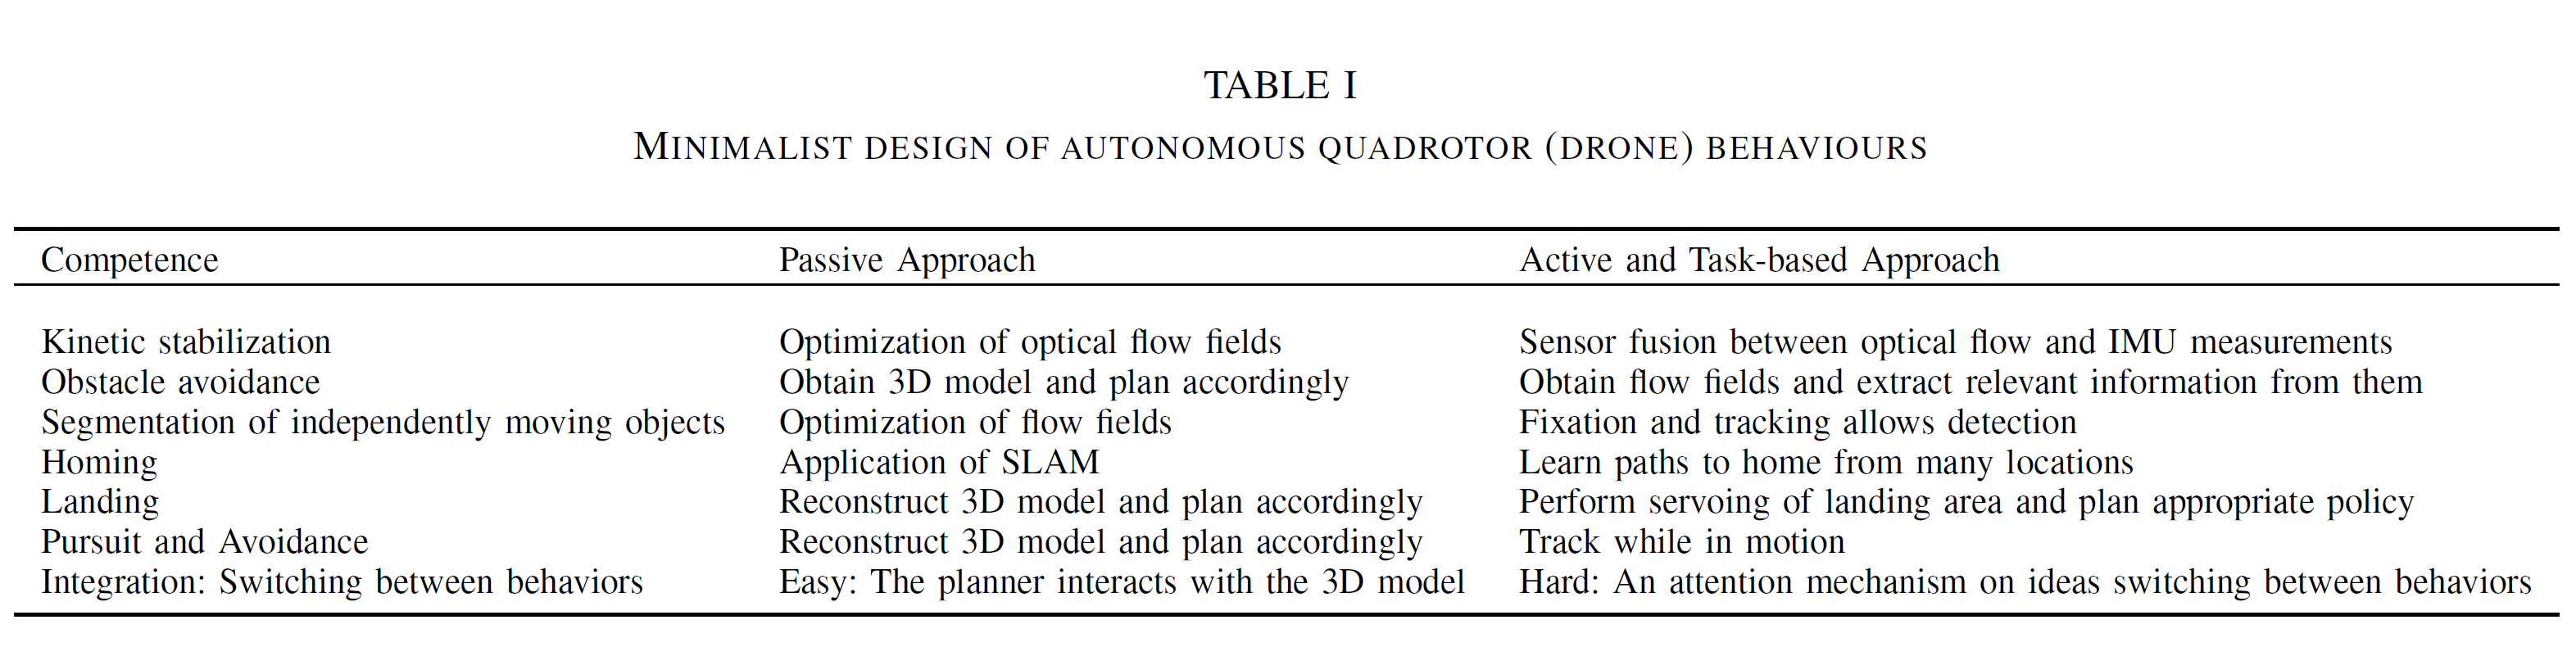
\includegraphics[width=1.0\textwidth]{../figures/table_1}
% 		\end{figure}
% 		\begin{itemize}
% 			\item Quadrotor "active" in nature
% 			\item Control image acquisition process
% 			\item Behaviors \only<2->{\textcolor{FIRE_BRICK}}{can be} accomplished without explicit 3D reconstruction
% 		\end{itemize}		
% 	\end{frame}

% 	\begin{frame}{Question and Key contributions}
% 		\only<2->{\textcolor{GRAY_WEB}}{\textit{“Can a quadrotor manage to go through an arbitrarily shaped gap without building an explicit 3D model of a scene, using only a monocular camera?”\\[10pt]}}
% 		\only<2>{\animategraphics[autoplay,loop,width=0.7\textwidth]{13.5}{../figures/gifs/drone_0/drone_0-}{0}{55}}
% 		\only<3->{
% 			\textbf{Key contributions}
% 			\begin{itemize}
% 				\item Active vision based structure-less minimalist gap detection algorithm \textemdash Temporally Stacked Spatial Parallax or TS\textsuperscript{2}P
% 				\item Visual servoing on a contour for the quadrotor to fly through unknown gaps
% 			\end{itemize}
% 		}
% 	\end{frame}
	


% % ------------------------------------------------------------------------------------------------- 
% % gap detection using TSSP
% % ------------------------------------------------------------------------------------------------- 

% \section[Gap Detection using TS\textsuperscript{2}P]{Gap Detection using TS\textsuperscript{2}P}
% \label{sec:gap_detection_using_tssp}

% 	\begin{frame}{Gap Detection using TS\textsuperscript{2}P}
% 		\only<1>{
% 			\animategraphics[autoplay,loop,width=0.8\textwidth]{13.5}{../figures/gifs/drone_1/drone_1-}{0}{55}}
% 		\only<2->{
% 		\begin{itemize}
% 			\item Optical flow
% 			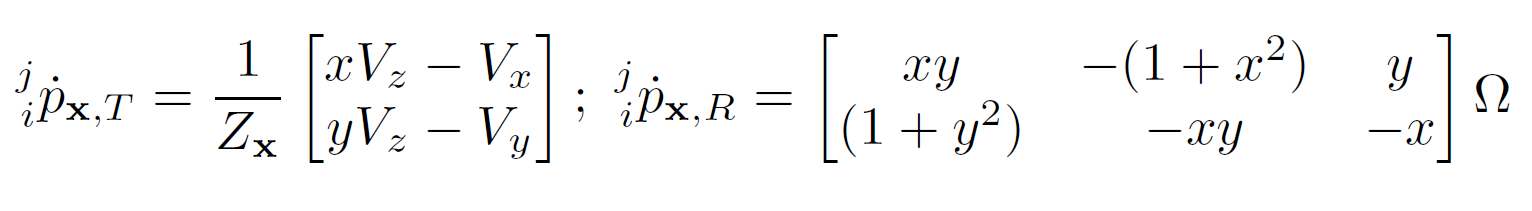
\includegraphics[width=1.0\textwidth]{../figures/e_of_1}
% 			\item Controlled motion
% 			
\includegraphics[width=1.0\textwidth]{../figures/e_2}
% 			\item Magnitude of optical flow can be given as 
% 			
\includegraphics[width=1.0\textwidth]{../figures/e_3}
% 		\end{itemize}
% 		}
% 	\end{frame}

% 	\begin{frame}{Gap Detection using TS\textsuperscript{2}P}
% 		\begin{itemize}
% 			\item<1-> To reduce noise
% 			
\includegraphics[width=1.0\textwidth]{../figures/e_4}
% 			\only<1>{
% 				\animategraphics[autoplay,loop,width=0.8\textwidth]{13.5}{../figures/gifs/drone_2/drone_2-}{0}{139}}
% 			\only<2->{
% 			\item Criterion for possible boundary region
% 			\begin{figure}
% 				\centering
% 				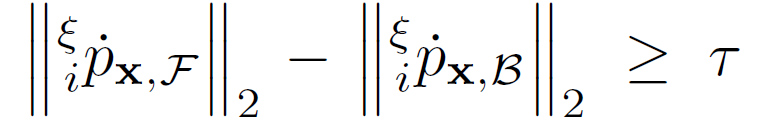
\includegraphics[width=0.5\textwidth]{../figures/e_5}
% 			\end{figure}
% 			\item Numerically stable \\
% 			\begin{figure}
% 				\centering
% 				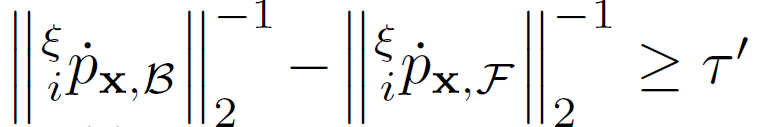
\includegraphics[width=0.5\textwidth]{../figures/e_6} \hfill
% 				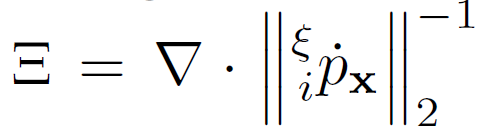
\includegraphics[width=0.3\textwidth]{../figures/e_7}
% 			\end{figure}
% 			}
% 		\end{itemize}
% 	\end{frame}



% % -------------------------------------------------------------------------------------------------
% % high speed gap tracking for visual servoing based control
% % -------------------------------------------------------------------------------------------------
% \section[High speed Gap Tracking for Visual Servoing based Control]{High speed Gap Tracking for Visual Servoing based Control}
% \label{sec:gap_tracking_visual_servoing}

% 	\begin{frame}{High speed Gap Tracking for Visual Servoing based Control}
% 		\only<1-3>{
% 			\begin{itemize}
% 				\only<1>{
% 					\item Focus of expansion (FOE)
% 					\begin{figure}
% 						\centering
% 						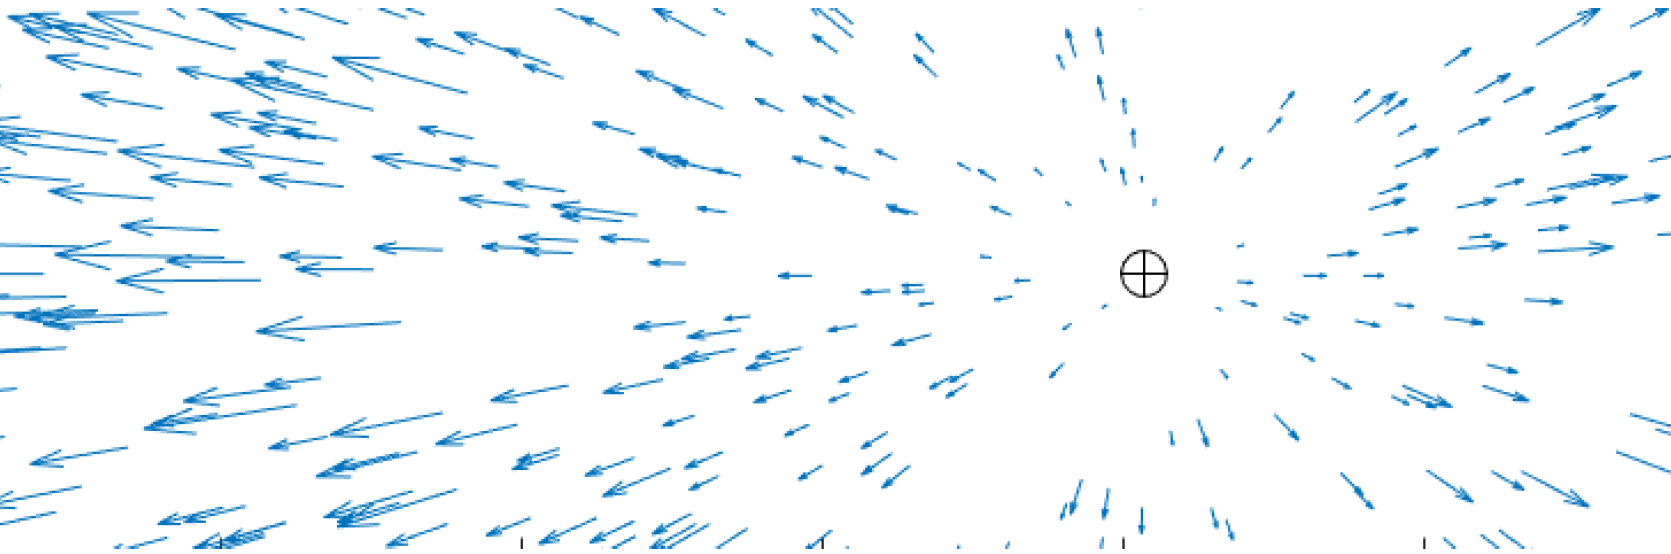
\includegraphics[width=0.7\textwidth]{../figures/foe_1}\\[10pt]
% 						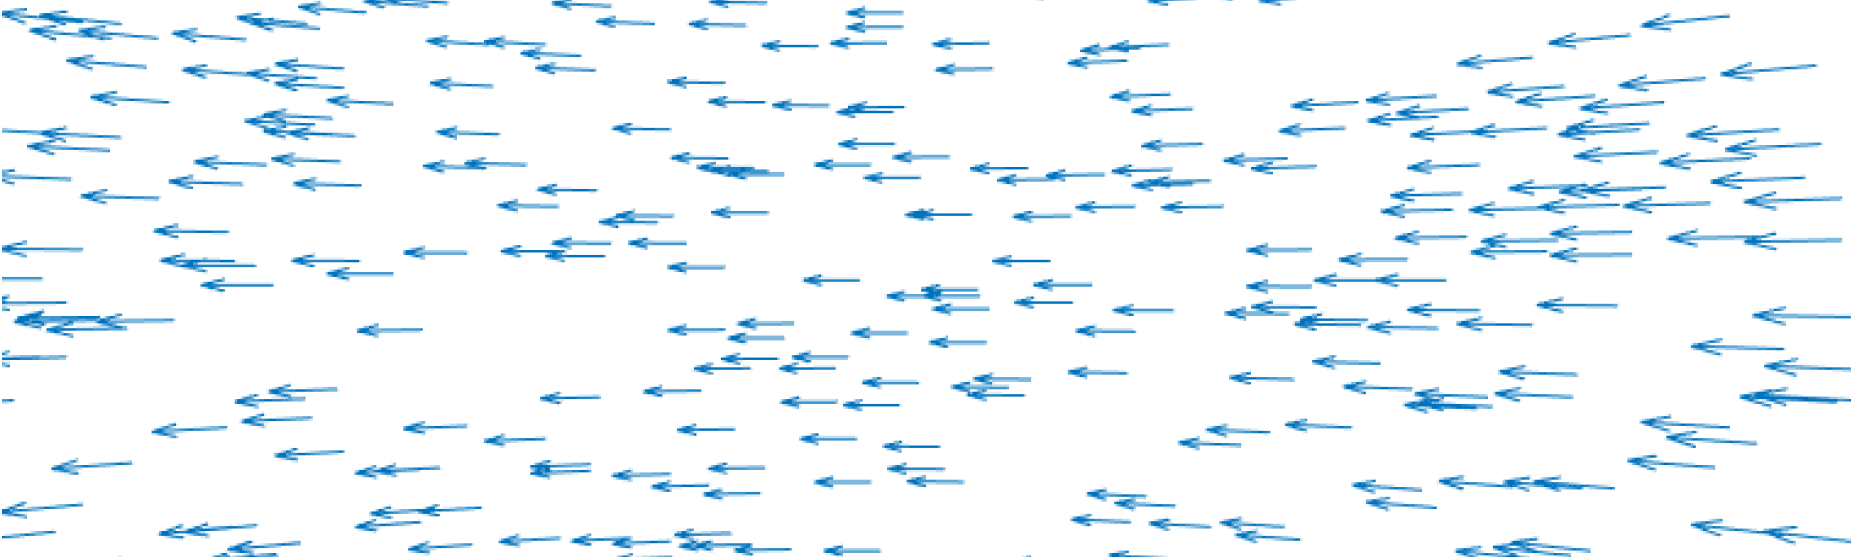
\includegraphics[width=0.7\textwidth]{../figures/foe_2}
% 					\end{figure}
% 				}
% 				\only<1-3>{\item Track a contour using label sets propagated using FOE}
% 				\only<2-3>{\item Each pixel associated with a score $\chi(\mathbf{x}) \in [-1, 1])$}
% 				\only<2-3>{
% 					\item $\mathcal{F} = \{\mathbf{x} \mid \chi(\mathbf{x}) = +1\}$, $\mathcal{B} = \{\mathbf{x} \mid \chi(\mathbf{x}) = -1\}$, $\mathcal{O} = \{\mathbf{x} \mid \chi(\mathbf{x}) < 0\}$, $\mathcal{C} = \{\mathbf{x} \mid \chi(\mathbf{x}) = 0\}$, $\mathcal{U} = \{\mathbf{x} \mid \chi(\mathbf{x}) \in (+1, -1)\}$
% 					\begin{figure}
% 						\centering
% 						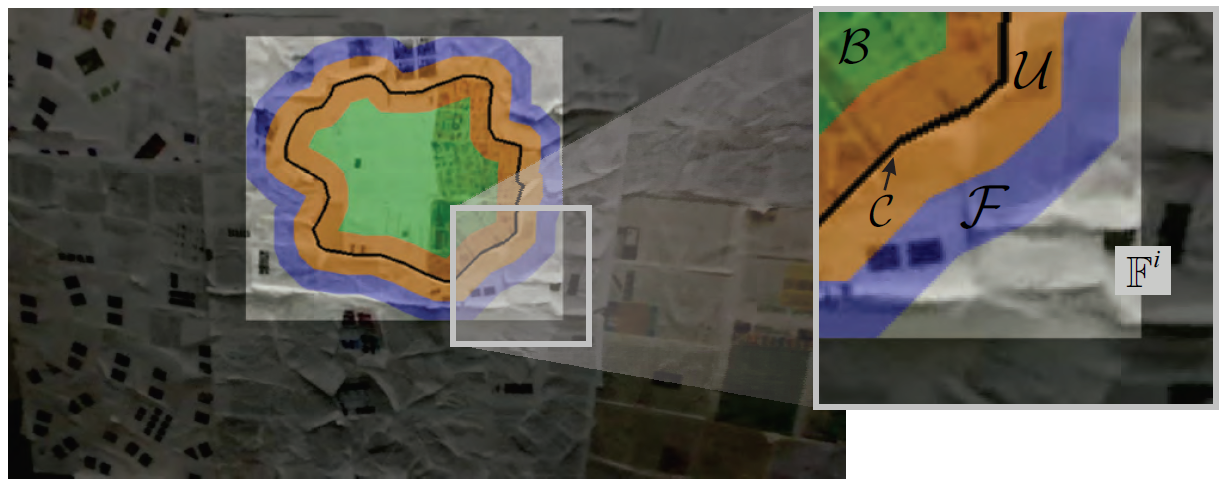
\includegraphics[width=0.5\textwidth]{../figures/labels_1}
% 					\end{figure}
% 				}
% 				\only<3>{\item<3> Track $\mathcal{F} \cup \mathcal{B}$ instead of $\mathcal{C}$}
% 			\end{itemize}
% 		}
% 		\only<4>{
% 			\begin{figure}
% 				\centering
% 				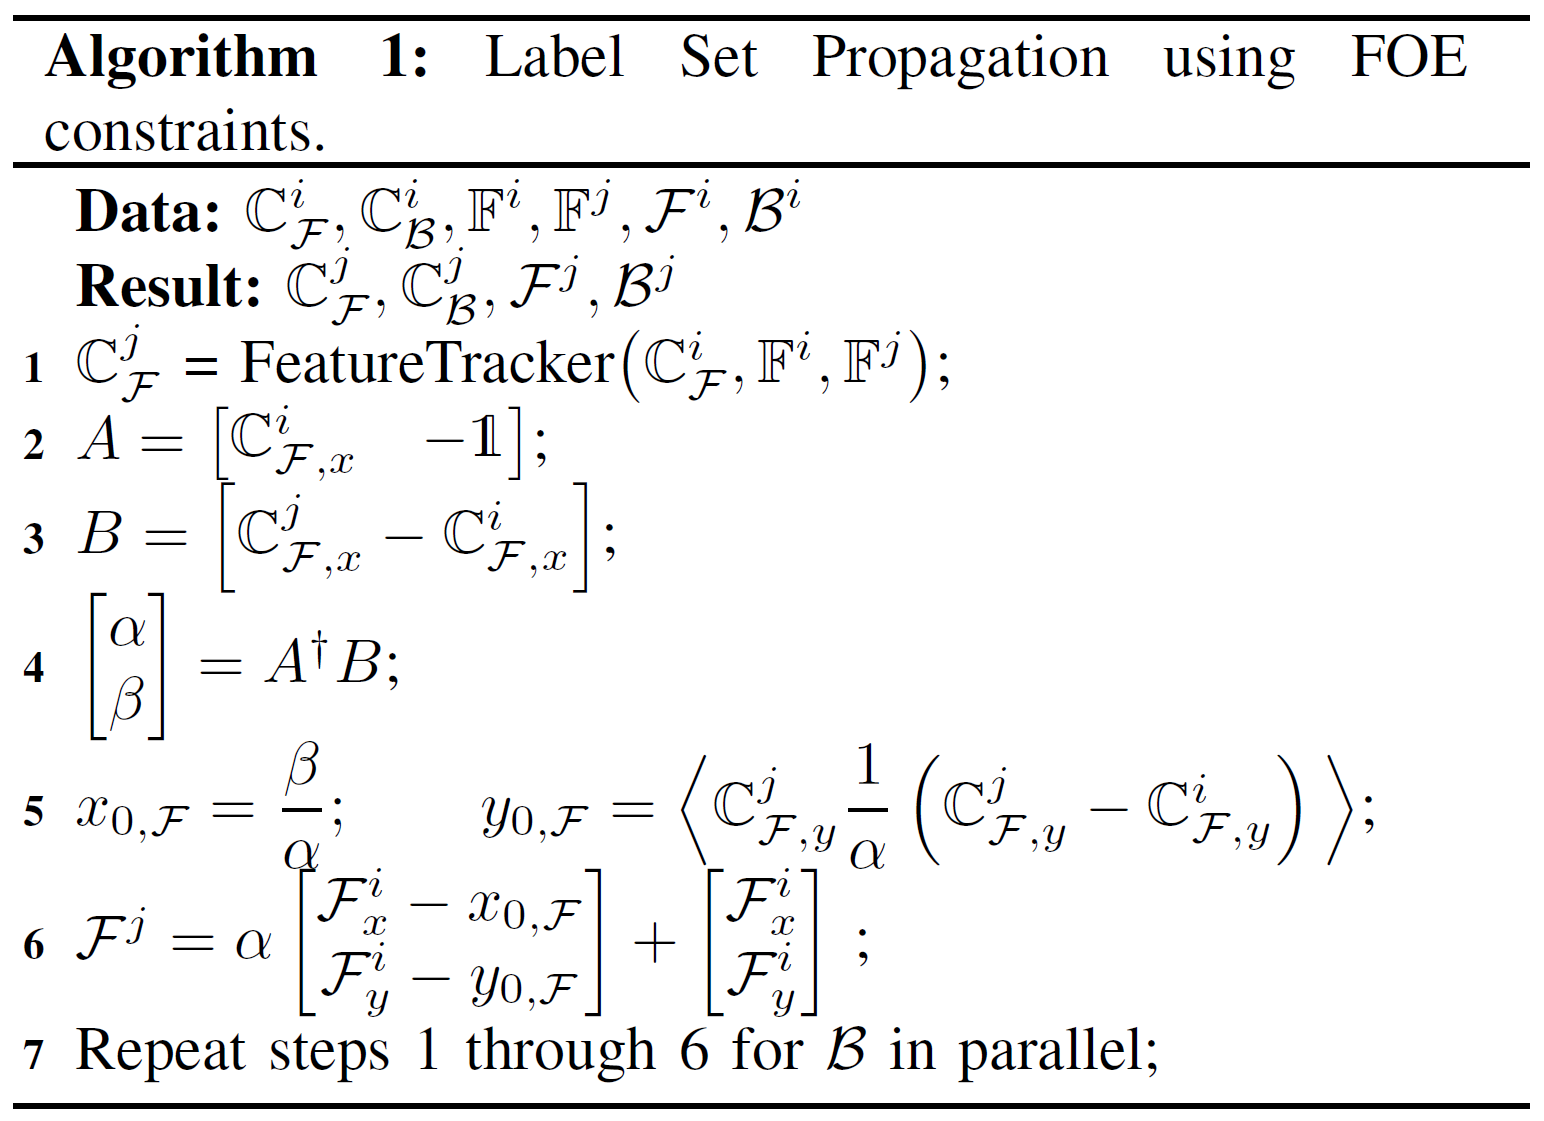
\includegraphics[width=0.8\textwidth]{../figures/algo}
% 			\end{figure}
% 		}
% 	\end{frame}

% 	\subsection[Safe Point Computation and Tracking]{Safe Point Computation and Tracking}
% 		\begin{frame}{Safe point Computation and Tracking}
% 			\begin{itemize}
% 				\only<1-2>{
% 					\item Quadrotor an ellipsoid
% 					\item Projection of quadrotor on image $\mathcal{Q} = \{\mathbf{x} \mid Q(\mathbf{x}) \leq 0\}$
% 					\item Safe region $\mathcal{S}$ 
% 					\begin{figure}
% 						\centering
% 						
\includegraphics[width=0.8\textwidth]{../figures/e_8}
% 					\end{figure}
% 				}
% 				\only<2>{
% 					\item Optimization problem becomes
% 					\begin{figure}
% 						\centering
% 						
\includegraphics[width=0.8\textwidth]{../figures/e_9}
% 					\end{figure}
% 					\item To favor less-aggressive maneuvers, regularization penalty
% 					\begin{figure}
% 						\centering
% 						
\includegraphics[width=0.8\textwidth]{../figures/e_10}
% 					\end{figure}
% 				}
% 				\only<3->{
% 					\item Simple efficient safe point computation
% 					\begin{figure}
% 						\centering
% 						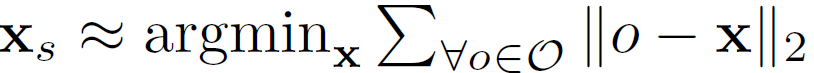
\includegraphics[width=0.5\textwidth]{../figures/e_11}
% 					\end{figure}
% 				}
% 				\only<4>{
% 					\begin{figure}
% 						\centering
% 						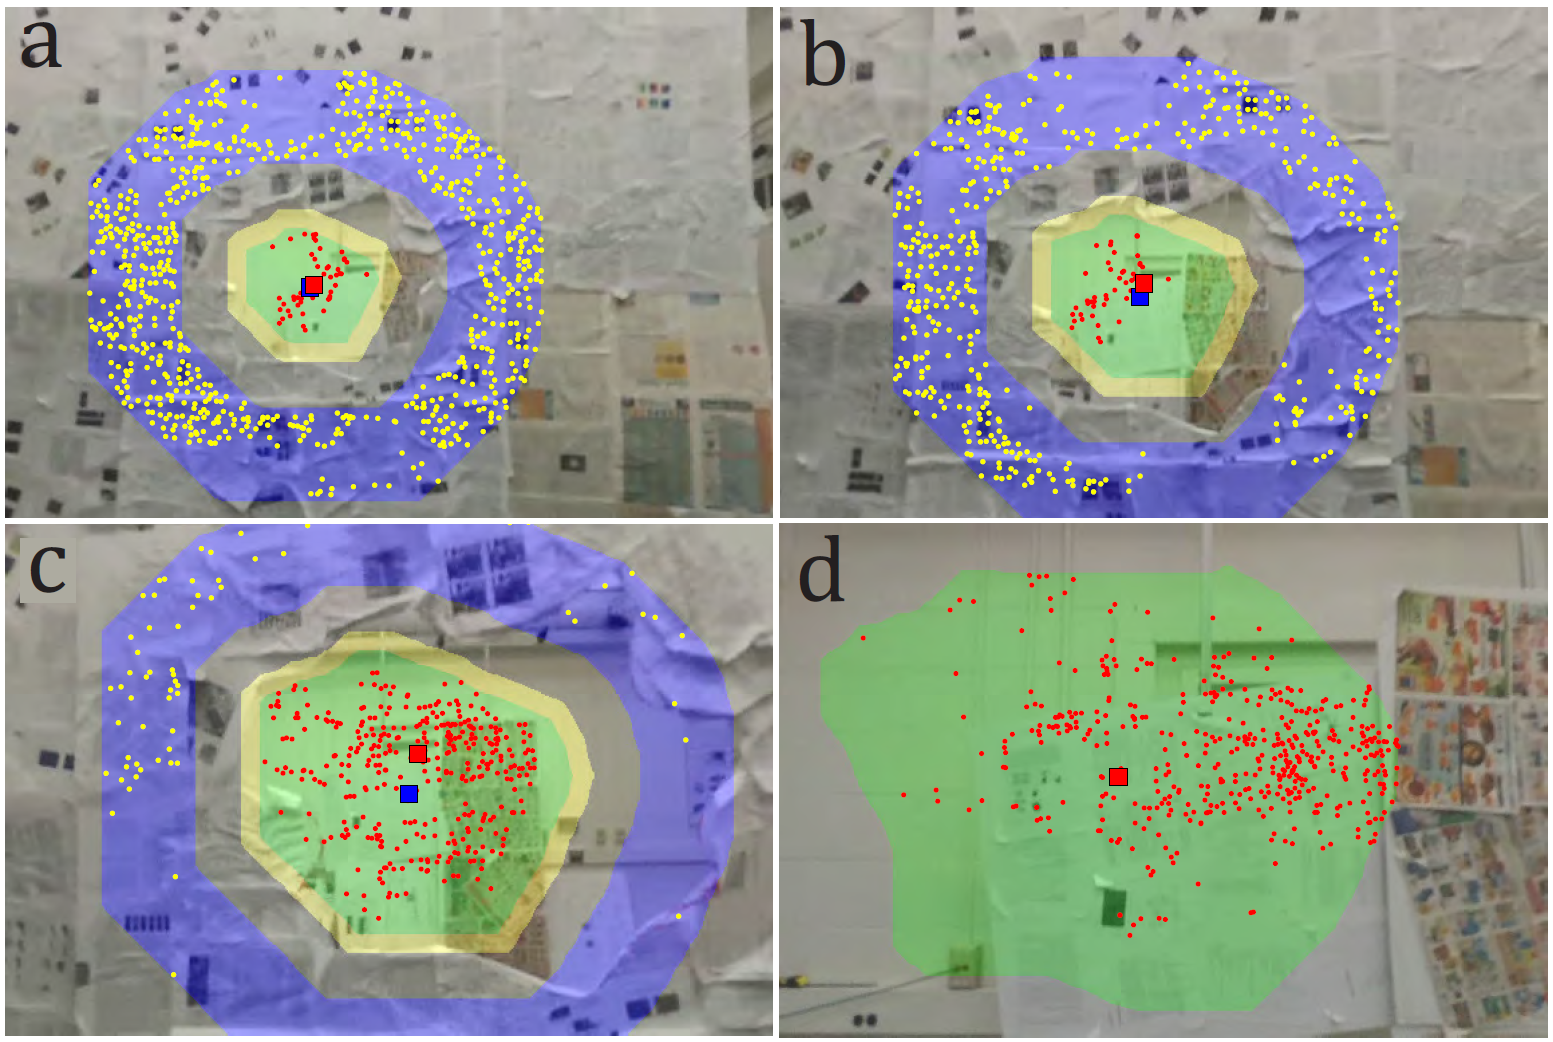
\includegraphics[width=0.8\textwidth]{../figures/safe}
% 					\end{figure}
% 				}
% 				\only<5>{
% 					\animategraphics[autoplay,loop,width=0.8\textwidth]{13.5}{../figures/gifs/drone_3/drone_3-}{0}{104}
% 				}
% 			\end{itemize}
% 		\end{frame}

% 	\subsection{Control Policy}
% 		\begin{frame}{Control Policy}
% 			\begin{itemize}
% 				\item Dynamic model adapted from \textit{"Minimum Snap Trajectories Generation and Control for Quadrotors, 2011"}
% 				\item Align projection of body center on image plane with $\mathbf{x}_s$
% 				\item Difference error $e$ is driven to $0$, simple PID
% 				\item Only lateral movements dealt
% 				\item Implicit assumption, gap is large enough 
% 			\end{itemize}
% 		\end{frame}



% % -------------------------------------------------------------------------------------------------
% % experiments
% % -------------------------------------------------------------------------------------------------
% \section{Experiments}
% \label{sec:experiments}

% 	\subsection{Experimental Setup}
% 	\begin{frame}{Experimental Setup}
% 		\only<1>{
% 			\begin{figure}
% 				\centering
% 				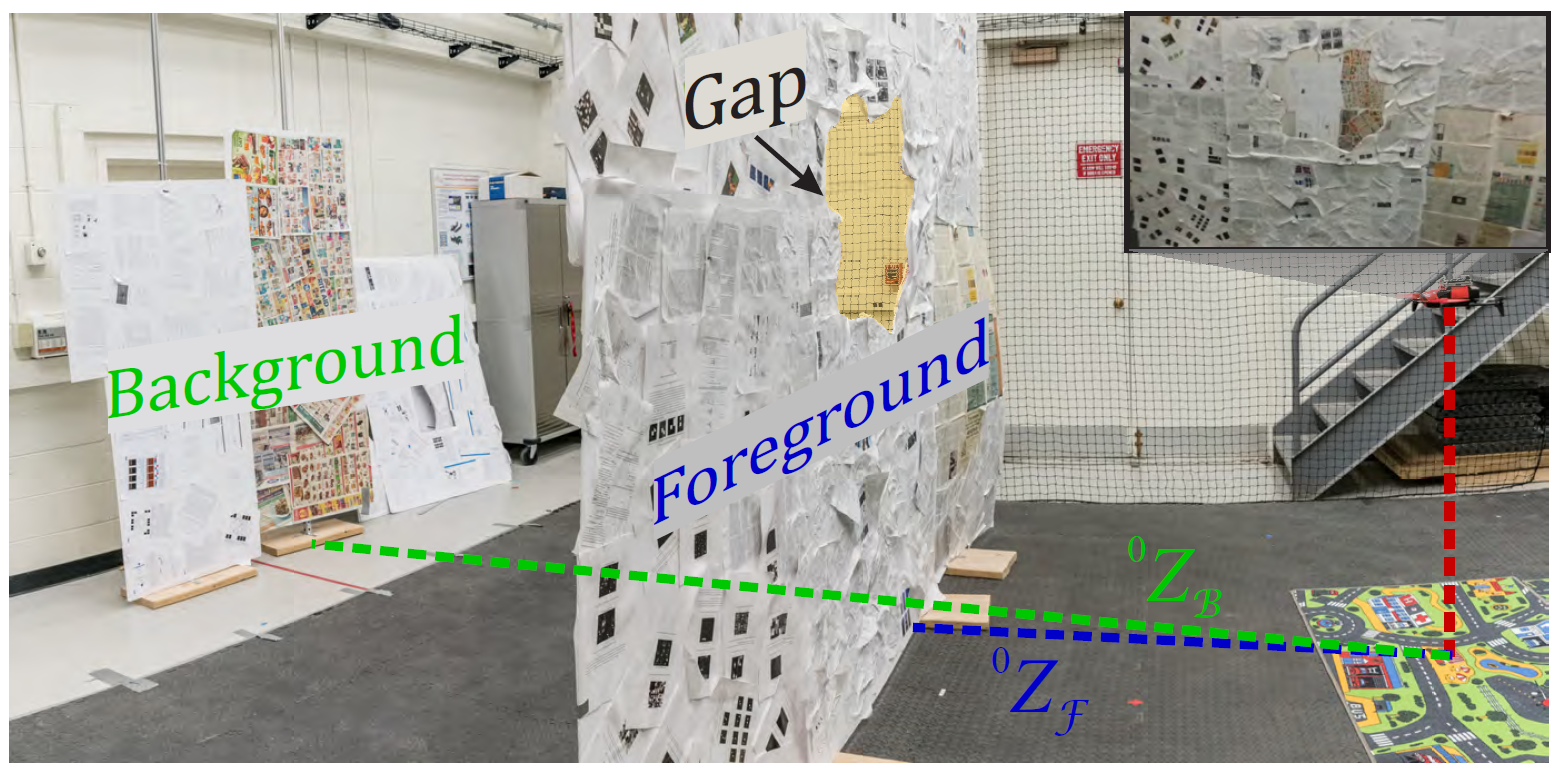
\includegraphics[width=0.8\textwidth]{../figures/gap_setup}
% 			\end{figure}
% 		}
% 		\only<2>{
% 			\begin{columns}
% 				\begin{column}[]{0.5\textwidth}
% 					\begin{itemize}
% 						\item Parrot Bebop 2 equipped with
% 						\begin{enumerate}
% 							\item font facing camera
% 							\item 9-axis IMU
% 							\item downward facing optical flow sensor
% 							\item coupled with sonar
% 						\end{enumerate}
% 						\item NVIDIA Jetson TX2 GPU
% 						\item TX2 Bebop communicate via WiFi
% 						\item Prototype MATLAB Robotics Toolbox
% 						\item Final versions, Python 
% 					\end{itemize}
% 				\end{column}
% 				\begin{column}[]{0.5\textwidth}
% 					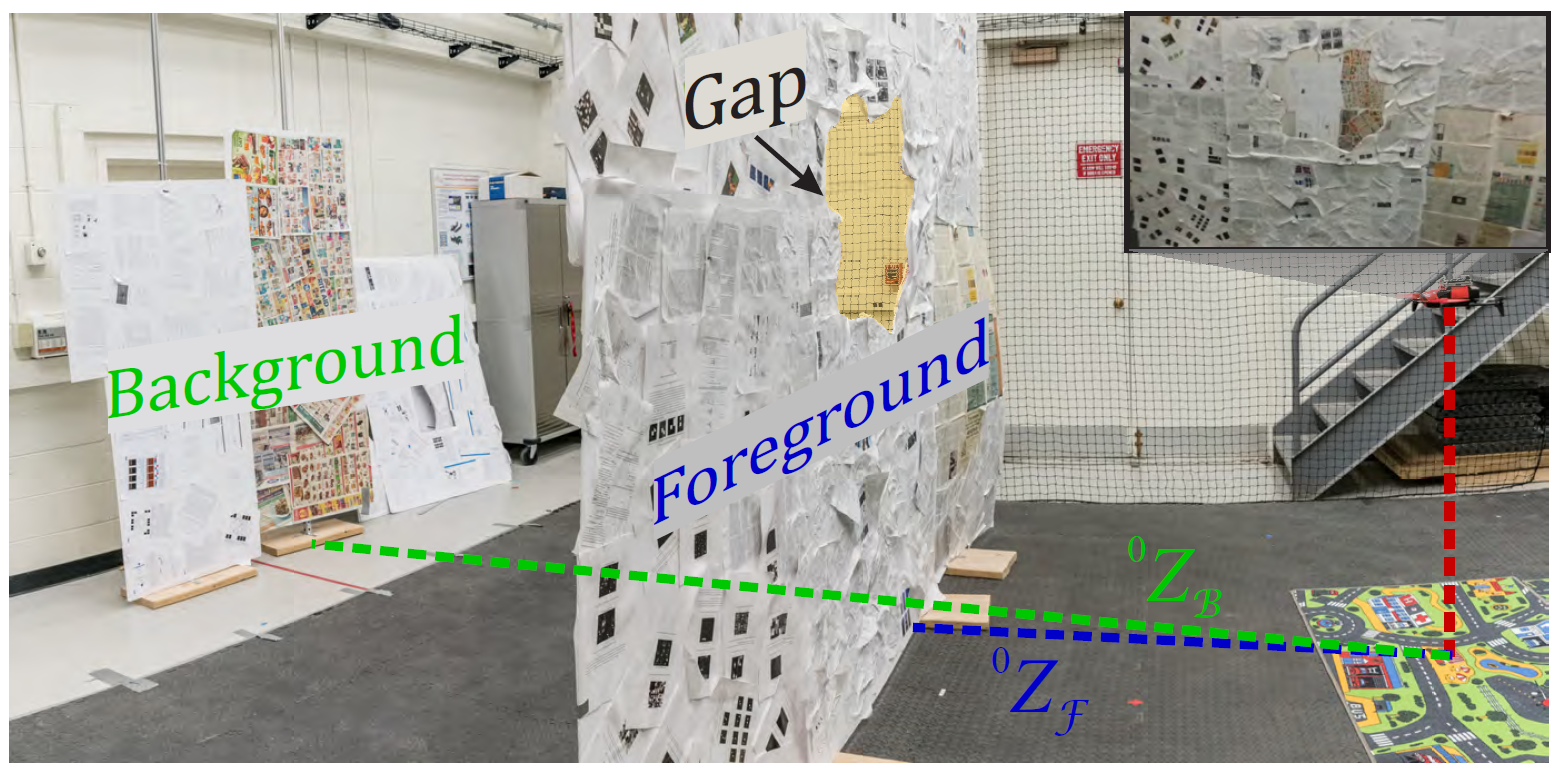
\includegraphics[width=0.8\textwidth]{../figures/gap_setup}
% 					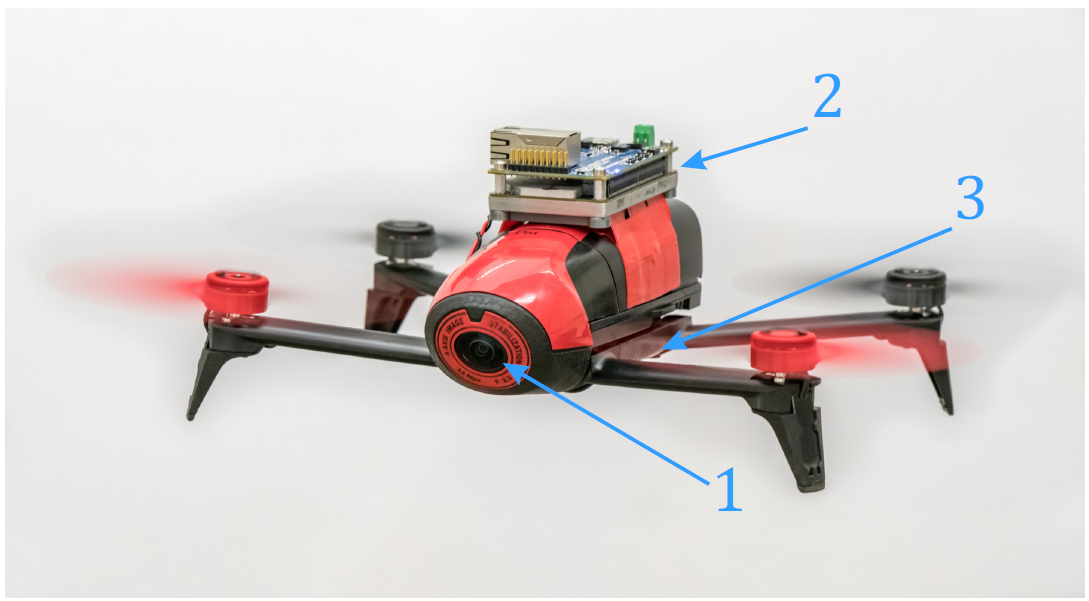
\includegraphics[width=0.8\textwidth]{../figures/parrot}
% 				\end{column}
% 			\end{columns}
% 		}
% 	\end{frame}

% 	\subsection{Experimental Results}
% 	\begin{frame}{Experimental Results}
% 		\only<1>{
% 			\begin{itemize}
% 				\item 1. Different arbitrarily shaped gaps
% 				\begin{figure}
% 					\centering
% 					\includegraphics[width=0.8\textwidth]{../figures/exp1.png}
% 				\end{figure}
% 			\end{itemize}
% 		}
% 		\only<2>{
% 			\begin{itemize}
% 				\item 2. Test noise sensitivity
% 				\begin{figure}
% 					\centering
% 					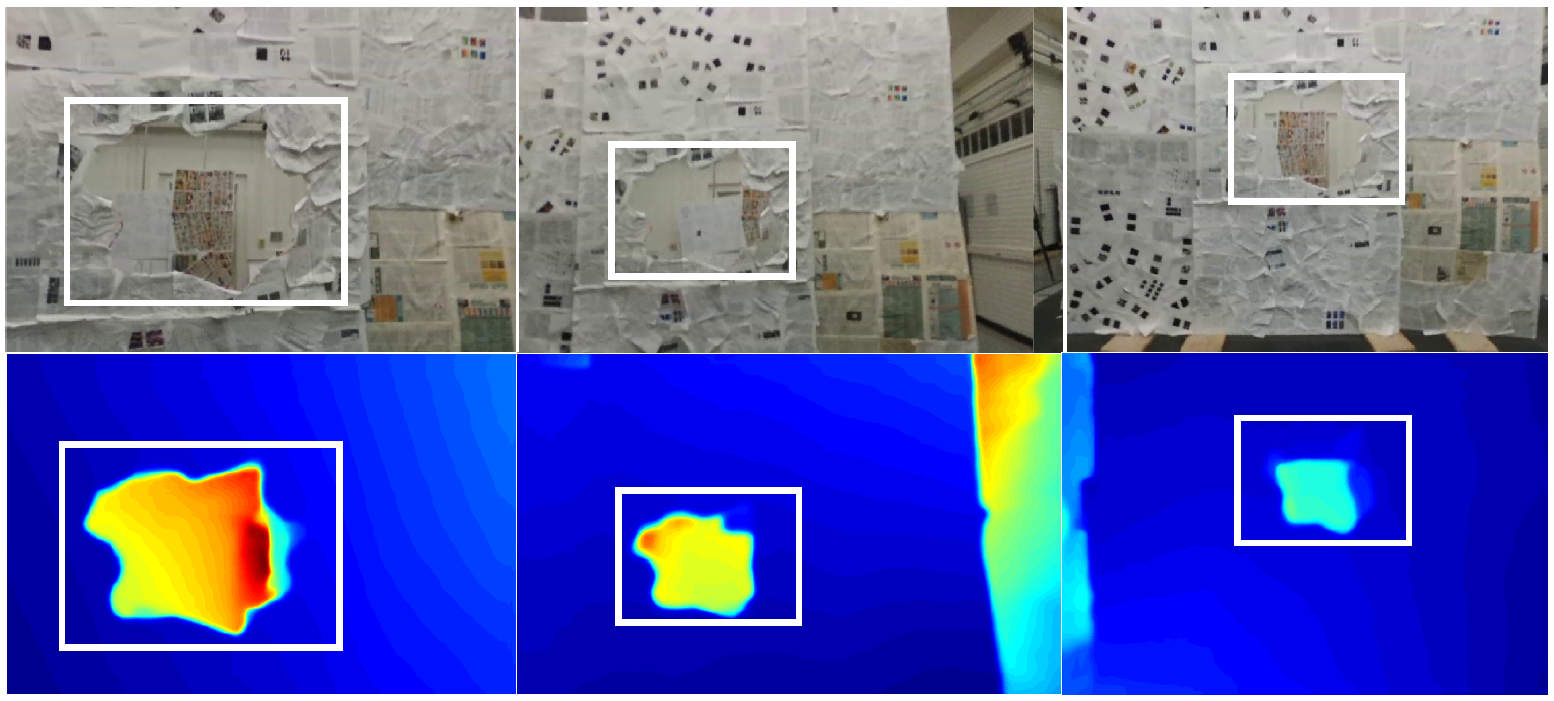
\includegraphics[width=0.8\textwidth]{../figures/exp2.png}
% 				\end{figure}
% 			\end{itemize}
% 		}
% 		\only<3>{
% 			\begin{itemize}
% 				\item 3. Different N, image baselines, image sizes
% 				\begin{figure}
% 					\centering
% 					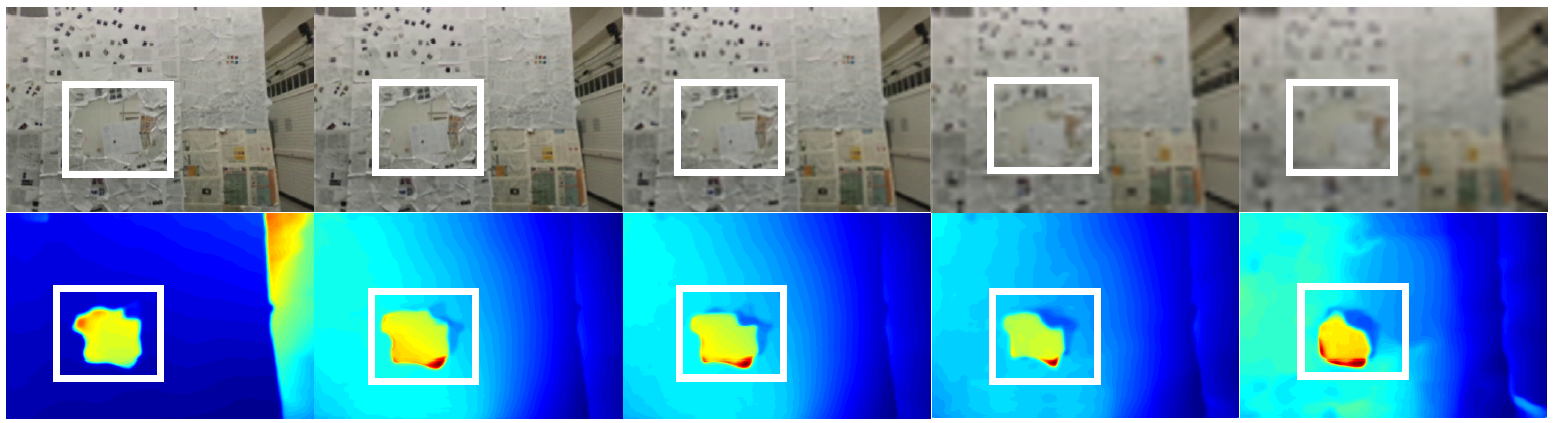
\includegraphics[width=0.8\textwidth]{../figures/exp_3_1.png}
% 					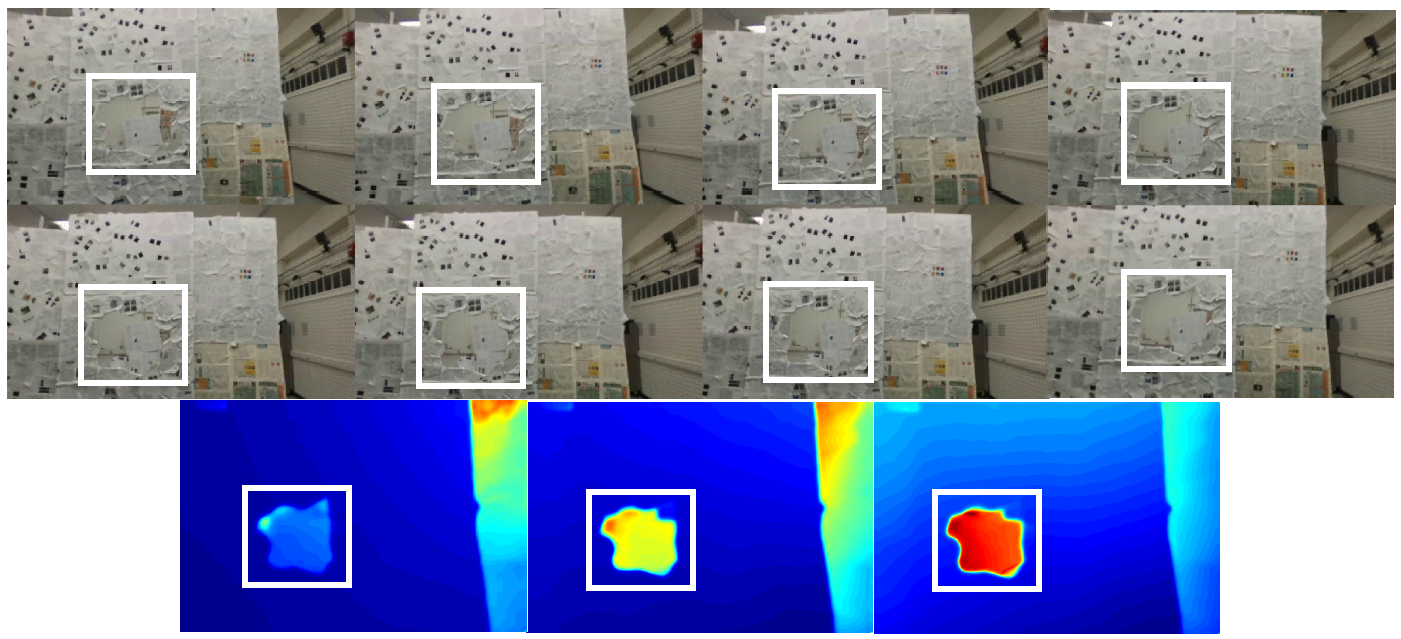
\includegraphics[width=0.8\textwidth]{../figures/exp_3_2.png}
% 				\end{figure}
% 			\end{itemize}
% 		}
% 		\only<4>{
% 			\begin{itemize}
% 				\item 4. Alternative approaches
% 				\begin{figure}
% 					\centering
% 					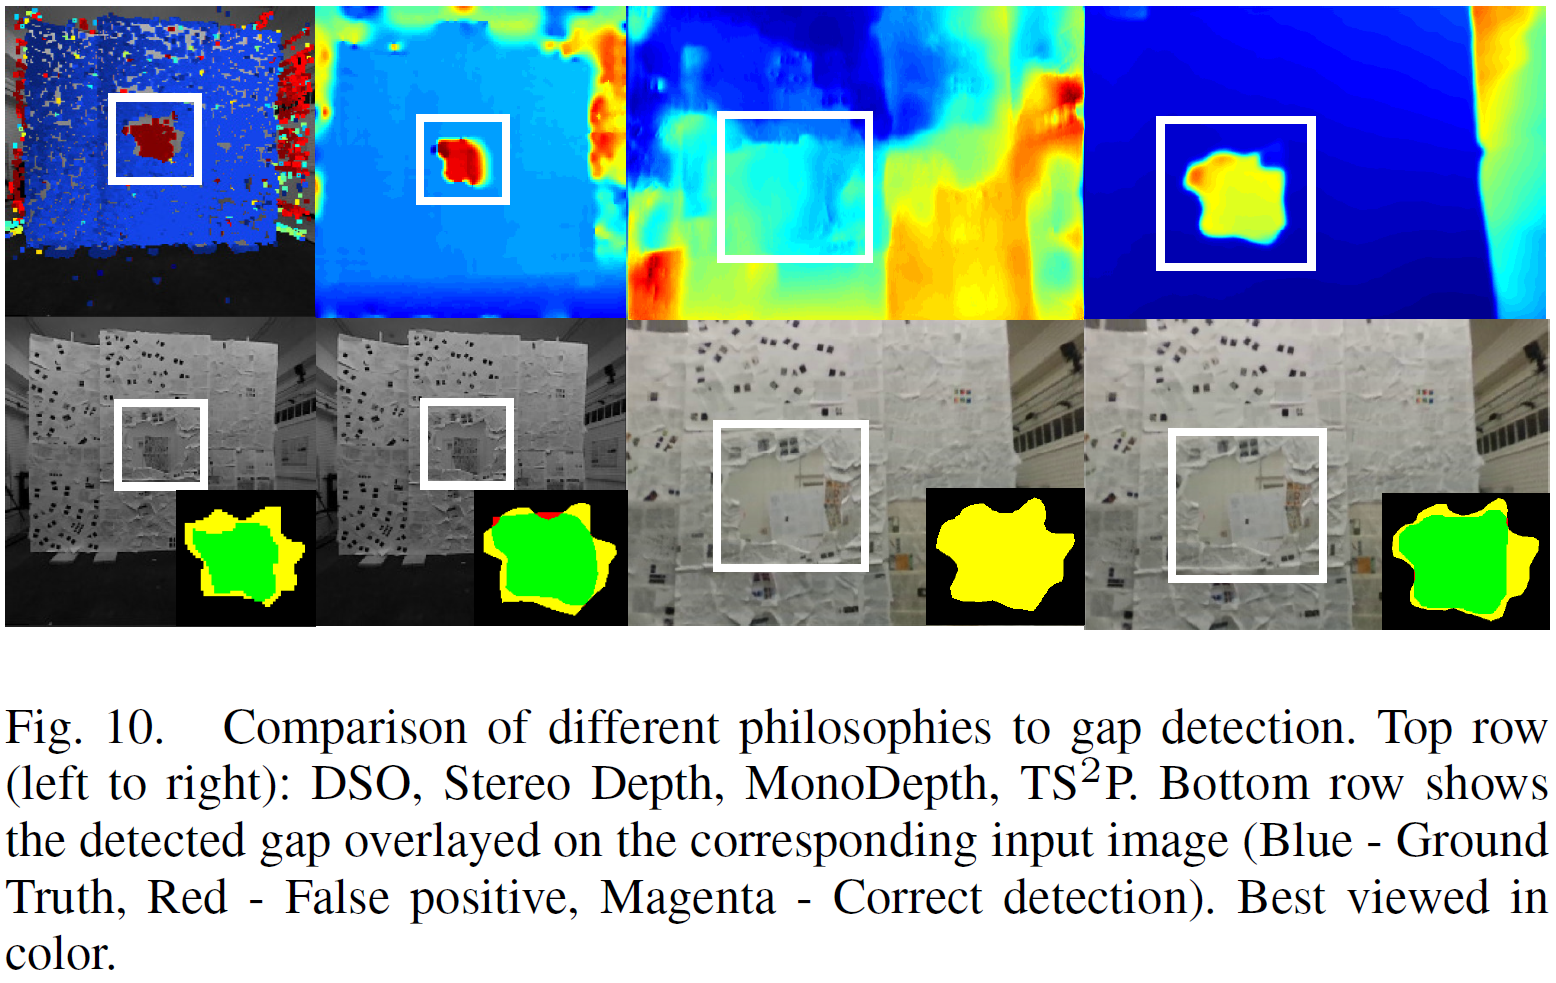
\includegraphics[width=0.8\textwidth]{../figures/exp4.png}
% 				\end{figure}
% 			\end{itemize}
% 		}
% 		\only<5>{
% 			\animategraphics[autoplay,loop,width=0.9\textwidth]{13.5}{../figures/gifs/drone_4/drone_4-}{0}{139}
% 		}
% 	\end{frame}


% % -------------------------------------------------------------------------------------------------
% % conclusion
% % -------------------------------------------------------------------------------------------------
% \section{Conclusion}
% \label{sec:conclusion}

% 	\begin{frame}{Conclusion}
% 		\begin{itemize}
% 			\item<1-> Minimalist philosophy mimicing Insects
% 			\item<2-> Solve complex problems with minimal sensing and active movement
% 			\item<3-> Philosophy used to find unknown gap using monocular camera and on board sensing
% 			\item<4-> Comprehensive comparisons and analysis provided
% 			\item<5-> Authors mention, \textit{to their knowledge this is the first paper to address gap detection of unknown shape and location with monocular camera and onboard sensing}
% 		\end{itemize}
		
% 	\end{frame}


% % -------------------------------------------------------------------------------------------------
% % extro
% % -------------------------------------------------------------------------------------------------
% 	\begin{frame}{Questions}
% 		\centering
% 		Thank you
% 	\end{frame}

\end{document}

